\documentclass{beamer}
\usetheme{Madrid}
\usepackage[utf8]{inputenc}
\usepackage[spanish]{babel}
\usepackage{amsmath}
\usepackage{amsfonts}
\usepackage{amssymb}
\usepackage{graphicx}
\usepackage{lipsum}
\usepackage{ragged2e}
\usepackage{hyperref}
\usepackage{float}
\usepackage{url}
\date{}

\definecolor{darkgreen}{RGB}{99, 111, 7}
\setbeamercolor{title}{fg=white,bg=darkgreen}

\begin{document}

\title[U CENTRAL]{} 
\author{JOSE A CARRILLO M \inst{1}} 
\logo{
\includegraphics[scale=0.2375]{sm.png}}


\begin{frame}
  \vspace{1cm}
  \centering
  {\Huge Estadística y Probabilidad }
  \vfill
  \begin{figure}[ht]
    \centering
    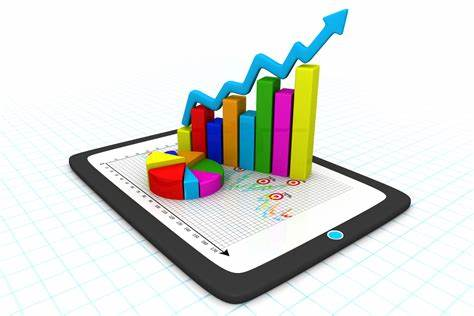
\includegraphics[width=0.5\textwidth]{imagen.png}
  \end{figure}
\end{frame}


\begin{frame}
\centering
\begin{beamercolorbox}[sep=8pt,center]{title}
{\Huge Estadística}
\usebeamerfont{title}\inserttitle\par%
\end{beamercolorbox}

\justify
\vspace{0.5cm}
La estadística es una rama de las matemáticas que se enfoca en la recolección, análisis e interpretación de datos "da sentido a los datos". 
\vspace{0.5cm}
Se utiliza en una amplia variedad de campos, como negocios, ciencia, tecnología, medicina, entre otros, para ayudar a tomar decisiones y hacer predicciones.
\end{frame}

\begin{frame}
\centering
\begin{beamercolorbox}[sep=8pt,center]{title}
{\Huge Probabilidad}
\usebeamerfont{title}\inserttitle\par%
\end{beamercolorbox}

\justify
\vspace{0.5cm}
Es una rama de las matemáticas que se encarga de cuantificar la posibilidad de que ocurra un evento o suceso determinado. En términos más simples, la probabilidad es la medida de la certeza o incertidumbre de que algo suceda.
\end{frame}

\begin{frame}
\frametitle{Ensayos clínicos}
\justify
Los ensayos clínicos son estudios de investigación que evalúan la eficacia y seguridad de nuevos tratamientos médicos en pacientes. La estadística se utiliza para diseñar ensayos clínicos y analizar los datos recopilados. Por ejemplo, se pueden usar pruebas estadísticas para determinar si un nuevo medicamento es más efectivo que un placebo.
\end{frame}

\begin{frame}
\frametitle{Epidemiología}
\justify
La epidemiología es el estudio de la distribución y los factores que influyen en la aparición y propagación de enfermedades en una población. La estadística se utiliza para analizar datos de salud y determinar las tasas de enfermedad, los factores de riesgo y los patrones de enfermedad en una población.
\end{frame}

\begin{frame}
\frametitle{Investigación genética}
\justify
La estadística se utiliza en la investigación genética para analizar datos de secuenciación de ADN y determinar la frecuencia de variantes genéticas en una población. La identificación y evaluación de biomarcadores potenciales también puede utilizar técnicas estadísticas para evaluar la capacidad predictiva de estos biomarcadores.
\end{frame}

\begin{frame}
\frametitle{La probabilidad en la medicina}

\begin{itemize}
\item La probabilidad es una herramienta importante en la medicina para:
\vspace{0.1cm}
\begin{itemize}
\item Estimar el riesgo de enfermedades
\item Tomar decisiones médicas informadas
\end{itemize}
\vspace{0.1cm}
\item Algunos ejemplos de uso de la probabilidad en la medicina son:
\vspace{0.1cm}
\begin{itemize}
\item Diagnóstico de enfermedades
\item Evaluación del riesgo
\item Toma de decisiones
\end{itemize}
\justify
\item Es importante recordar que la probabilidad solo puede proporcionar una estimación del riesgo y que los médicos deben utilizar su experiencia clínica y el juicio para tomar decisiones informadas y personalizadas para cada paciente.
\end{itemize}
\end{frame}


\begin{frame}
\frametitle{Analítica}
\justify
La estadística y la probabilidad son herramientas esenciales, la estadística ayuda a resumir y describir los datos, así como a identificar patrones y tendencias. Se utilizan para hacer inferencias sobre poblaciones basándose en muestras de datos, proporcionar una base sólida para la toma de decisiones informadas.

\vspace{0.5cm}
\justify
La probabilidad se utiliza en el análisis de datos para modelar eventos aleatorios y para predecir resultados futuros basados en eventos pasados. 
\end{frame}

\begin{frame}
\centering
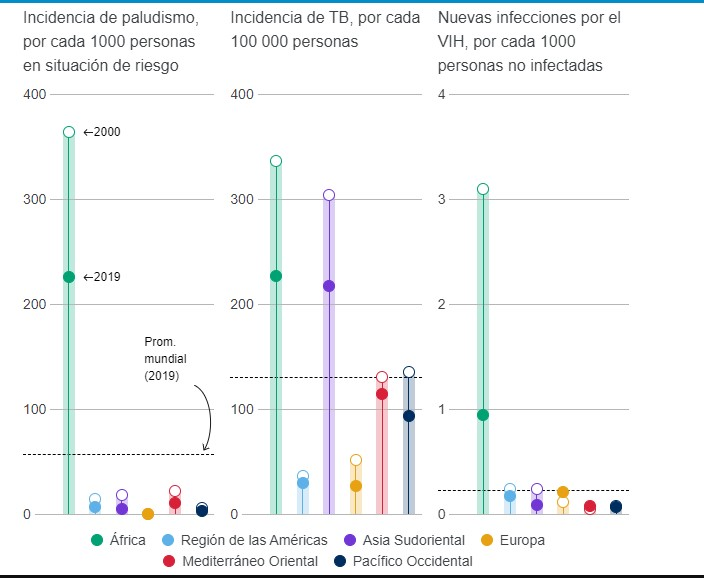
\includegraphics[width=0.8\textwidth]{oms.jpg}
\begin{beamercolorbox}[sep=1em,wd=\paperwidth,rightskip=0.5cm]{footline}
Recuperado de: OMS https://www.who.int/es
\end{beamercolorbox}
\end{frame}


\begin{frame}
\frametitle{Referencias}
\begin{itemize}
\item World Health Organization. (2021). World Health Statistics 2021: A Visual Summary [Datos resumidos visuales]. https://www.who.int/es/data/stories/world-health-statistics-2021-a-visual-summary 
\vspace{0.1cm}
\itemBencardino, C. M. (2019). Estadística básica aplicada. Ecoe Ediciones.
\vspace{0.1cm}
\item The Lancet. (s. f.). Inicio. Recuperado el 19 de febrero de 2023, de https://www.thelancet.com/
\vspace{0.1cm}
\item PubMed. (s. f.). Estudios de estadística. Recuperado el 19 de febrero de 2023, de https://pubmed.ncbi.nlm.nih.gov/?term=estudios+de+estadistica
\vspace{0.1cm}
\item Walpole, R. E., Myers, R. H., Myers, S. L., & Cruz, R. (1992). Probabilidad y estadística (Vol. 624). México: McGraw-Hill.
\vspace{0.1cm}
\item Cáceres, R. Á. (2007). Estadística aplicada a las ciencias de la salud. Ediciones Díaz de Santos
\vspace{0.1cm}
\end{itemize}
\end{frame}


\end{document}